% methodology

\section{Introduction}

The previous chapter expressed a number of propositions around autonomous motivation, cognition\hyp{}based trust, and power that may possibly shape tacit knowledge sharing relations in open innovation partnerships. This chapter details the mixed\hyp{}method social network analysis approach used to evaluate these propositions. \medskip

The chapter begins by explaining the rationale for a hybrid mixed\hyp{}method research design used in this study. This includes the argument for embracing pragmatist worldview and the motivation for combining key elements of  \enquote{convergent\hyp{}parallel} and \enquote{sequential\hyp{}explanatory} research in a hybrid research design. The chapter then details the quantitative and qualitative procedures used to collect and analyse data in this study. Finally, the chapter explains how the quantitative and qualitative strands were merged to provide a more nuanced view of tacit knowledge sharing in open innovation partnerships. \medskip

\section{Hybrid mixed\hyp{}method research design}

\subsection{Philosophical approach}

Philosophical debates tend to revolve around \enquote{ontology} and \enquote{epistemology}. Ontology refers to the nature of reality whereas epistemology is about the theory of knowledge used to make sense of reality. Treating reality as concrete is appropriate when dealing with the physical world. However, when considering human behaviour, reality is what people make it out to be. Researchers investigating physical phenomena are inclined to embrace a positivist worldview. They see themselves as detached observers, able to reduce a problem into measurable and unambiguous parts, and demonstrate causality through statistical and mathematical methods \citep{easterby2015management}. Researchers studying human behaviour, on the other hand, are more likely to embrace a constructivist worldview that can deal with complexity borne out of multiple realities. Though positivist and constructivist worldviews are fundamentally different, both worldviews place great emphasis on the research method used to guide inquiry \citep{easterby2015management}. \medskip

The author was motivated to study open innovation because of an innate desire to become a more effective research manager. He wanted to understand how one can deliver more radical innovations through collaborative research and development. Given all knowledge is contingent on the interests of those creating it, the tools and procedures they use to measure the phenomena under investigation, and the analytic frameworks they use to interpret their results \citep{monahan2010benefits}, the author did not think a post-positivist approach was appropriate for this study. His philosophical world-view is one of pragmatism, which is primarily concerned with actions, situations and consequences, rather than antecedent conditions \citep{creswell2013research}. \medskip

\begin{table}[]
    \centering
    \caption{Different philosophical world-views \citep{creswell2011designing}.}
    \label{tab:worldview}
    \begin{adjustbox}{width = \textwidth}
        \begin{tabular}{@{}l | cccc@{}}
            \toprule
             & Positivism & Constructivism & Participatory & Pragmatism \\ \midrule
            Ontology & Single reality & Multiple realities & Political reality & Single and multiple realities \\
            Epistemology & Distance and impartiality & Closeness & Collaborative & Practical \\
            Axiology & Unbiased & Biased & Negotiated & Multiple stances \\
            Methodology & Deductive & Inductive & Participatory & Combinatorial \\
            Rhetoric & Formal & Informal & Advocacy & Formal or informal \\ \bottomrule
        \end{tabular}
    \end{adjustbox}
\end{table}

Table \ref{tab:worldview} highlights the key differences between positivist, constructivist, participatory, and pragmatist worldviews. What is appealing about pragmatism is its practicality, not so much its broader philosophical basis \citep{morgan2014pragmatism}. Pragmatism can deal with more than one reality, is not confined to a specific viewpoint, and is able to handle multiple or mixed methods \citep{johnson2004mixed}. With mixed methods, the researcher works under the assumption that collecting diverse data provides a more complete understanding of the research problem than what can be provided by either quantitative or qualitative research alone \citep{creswell2013research}. How this works in practice is that the researcher gathers both close-ended quantitative and open-ended qualitative data, integrates the two, and then draws interpretations based on the combined strengths of both sets of data to better understand the research problem \citep{creswell2011designing}. \medskip

\subsection{Mixed-methods research design}

This study is cross\hyp{}sectional in nature and case\hyp{}based. Though a longitudinal study would provide fascinating insights into the evolution of an open innovation partnership, undertaking such a study for a PhD is unrealistic. Very few partnerships would be willing to commit to an intrusive longitudinal study. For the sake of expediency, the author decided to go with a cross-sectional, cased-based, study. A case\hyp{}based approach seeks understanding of a social situation or process by focusing on how it is played out in one or more bounded cases \citep{richards2012readme}. Our goal in this study is to seek a better understanding of knowledge sharing processes in three open innovation partnerships (cases). \medskip

Each case employs the same hybrid mixed-method research design, one that combines elements from a convergent\hyp{}parallel and a sequential\hyp{}explantory mixed\hyp{}method research design (Figure \ref{fig:design}). A convergent\hyp{}parallel design collects quantitative and qualitative data, analyses both data sets, and then merges the results of the two sets of data analyses with the purpose of comparing the results to gain a more complete understanding of the research problem \citep{creswell2014concise}. With an explanatory\hyp{}sequential design, the intent is to first use quantitative methods and then use qualitative methods to help explain the quantitative results in more depth \citep{creswell2014concise}. \medskip

\begin{figure}
    \centering
    \label{design}
    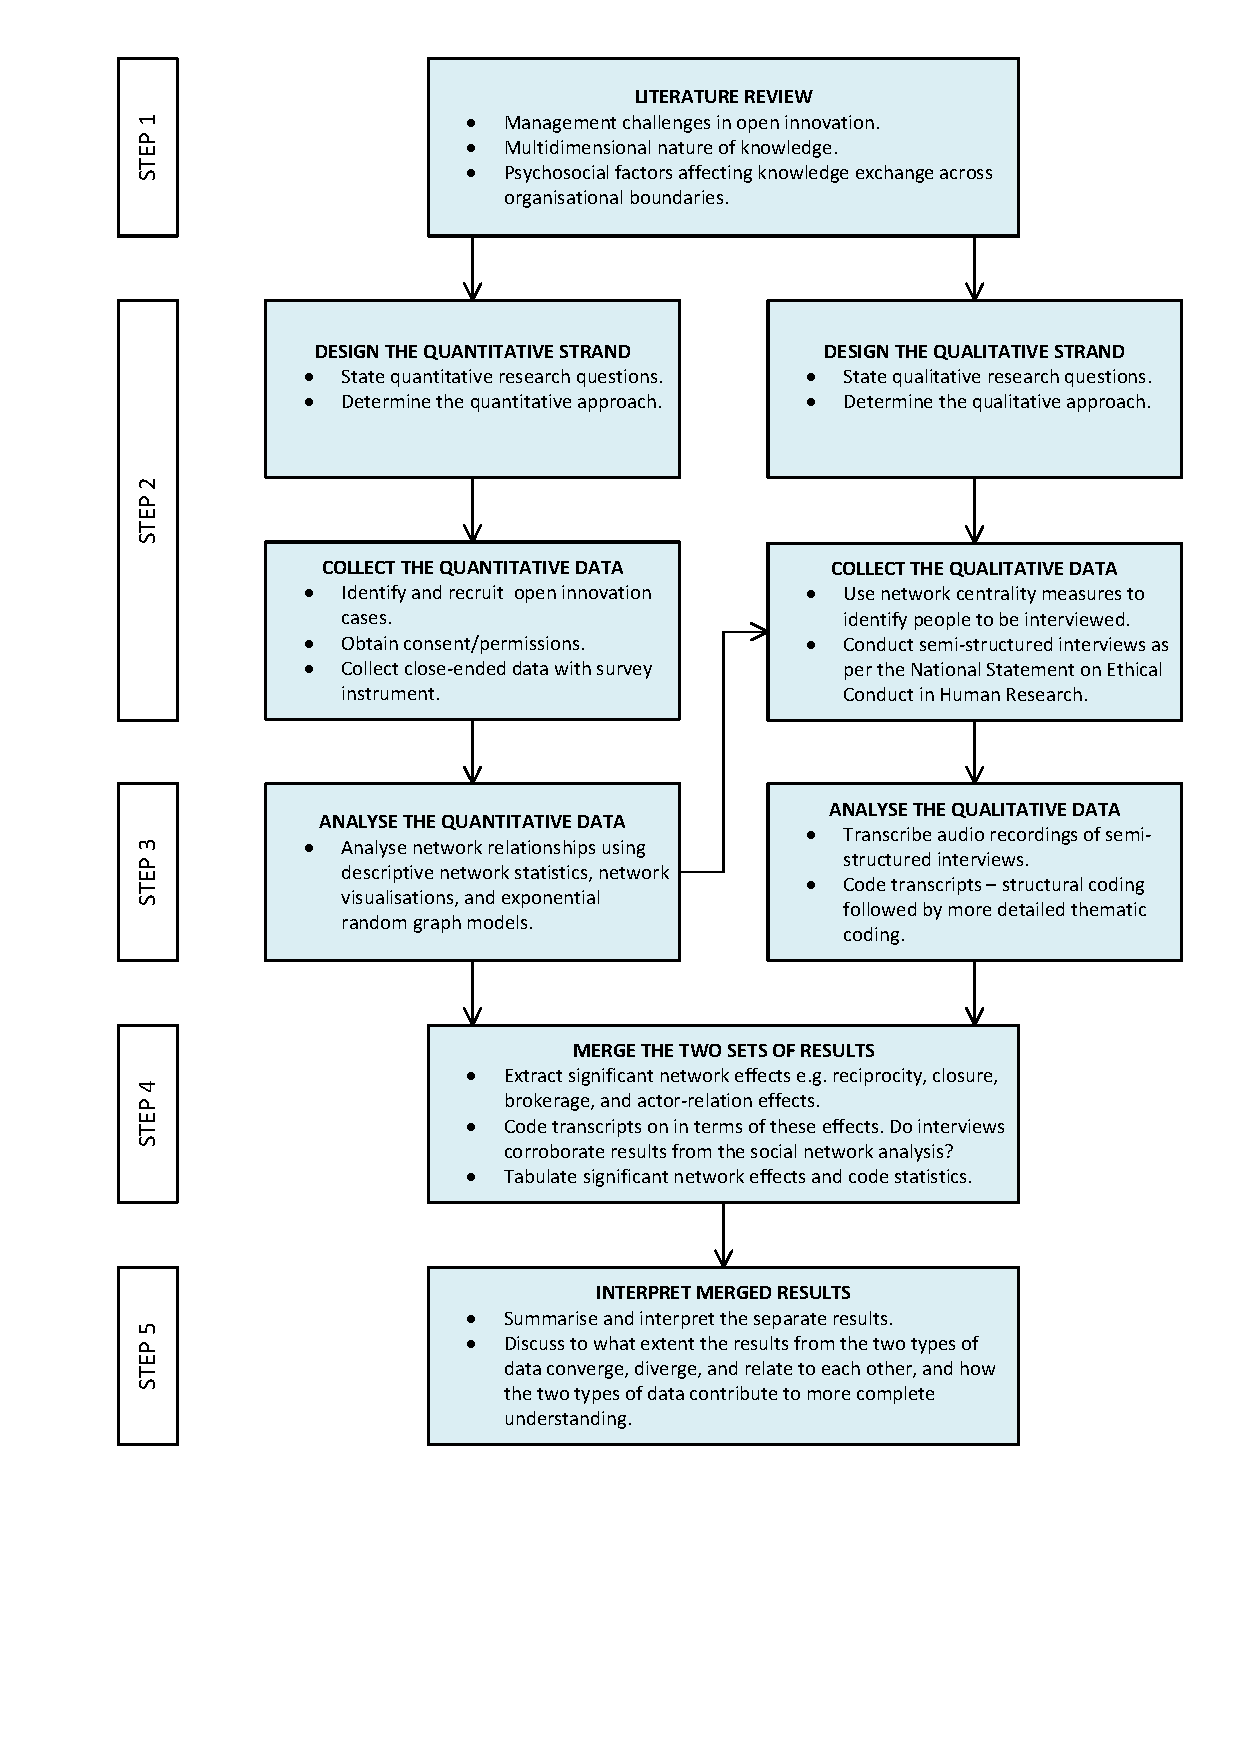
\includegraphics[width=0.9\linewidth]{Images/MixedMethodDesign20180903.pdf}
    \caption{Mixed\hyp{}method research design used in this study}
    \label{fig:researchplan20160402}
\end{figure}

The study initially considered employing a explanatory\hyp{}sequential design only, but in the interests of time and desire to reduce impositions on research participants, a decision was made to collect qualitative data in parallel with the quantitative analysis. Since one aim of this study was to gain insight into the environmental factors governing the emergence tacit knowledge sharing relations, the decision to collect contextual data in parallel with the quantitative analysis is reasonable. That said, the research design is weighted towards a sequential\hyp{}explanatory approach and does prioritise the quantitative strand over the qualitative strand. \medskip

The prioritisation of the quantitative strand is justified by the type of social network analysis being performed. This study uses exponential random graph modelling to assess patterns of social interaction. Exponential random graph models are a class of statistical model for social networks able to address complex social structures and unpack competing explanations for the presence (or absence) of network structures \citep{lusher2013exponential}. Unlike conventional social network analysis, exponential random graph models allow a researcher to simultaneously test multiple hypotheses or propositions about network tie formation relating to social theory \citep{robins2007recent}. The analytical power of exponential random graph models justifies the prioritisation of the quantitative strand over the qualitative strand. \medskip

A key challenge in any mixed\hyp{}method research design is the methodology used to merge the quantitative and qualitative strands \citep{ostlund2011combining}. In this study, the quantitative and qualitative strands are integrated at the point of data collection (where the quantitative results informed which individuals or actors should be prioritised for semi-structured interviews) and at the point of data interpretation (where the semi-structured interviews are used to make sense of the social network analysis results). This study uses \enquote{methodological triangulation} to integrate the quantitative and qualitative strands at the point of data interpretation \citep{denzin1994handbook}. No attempt was made to triangulate the three case studies as each open innovation partnership is quite unique and at a different stage of development (see Figure \ref{cases} below). The triangulation focuses on achieving a more complete picture of tacit knowledge sharing, rather than attempting to validate one set of results with another \citep{adami2005use}. Figure \ref{fig:triangulation} illustrates how the triangulation for completeness was applied in this study \citep{ostlund2011combining}. \medskip

% \begin{figure}
%     \centering
%     \label{design}
%     \includegraphics[width=0.9\linewidth]{Images/MixedMethodTriangulation.pdf}
%     \caption{Mixed\hyp{}method research design used in this study}
%     \label{fig:triangulation}
% \end{figure}

Whereas results from multiple\hyp{}case research are more easily generalised and better grounded than those of single\hyp{}case studies, drawing meaningful conclusions from cross\hyp{}sectional data collected in different contexts is a challenge \citep{eisenhardt2007theory}. Notwithstanding this challenge, the hybrid research design will still deliver rich insights into the processes of knowledge sharing and idea generation in open innovation partnerships \citep{walsham1995interpretive}. \medskip

\section{Ethics clearance}

Because this study deals with human subjects and involves commercially sensitive information, it was subject to the ethical guidelines contained in the Australian National Statement on Ethical Conduct in Human Research \citep{national2007national}. Data could not be collected without formal ethics approval from both the Commonwealth Scientific and Industrial Research Organisation and Swinburne University of Technology. Approval hinged on individual participants being sufficiently informed to give consent, allowing information about themselves to be used in this study. An application for ethics clearance was submitted to the ethics committees at both organisations. The application included a brief description of this study, a plain language information sheet for participants, a blank consent form, and a list of questions to be included in an on-line survey. Both committees deemed this study low\hyp{}risk and allowed the collection and subsequent analysis of data to proceed, subject to standard terms and conditions as per the National Statement on Ethical Conduct in Human Research. These include alerting both committees to any changes in data collection procedures and reporting any complaints or issues raised by participants. While some individuals chose not to participate in this study, none of those who agreed to participate raised any complaints or issues with the way this study was conducted. No changes were made to data collection procedures. \medskip

\section{Research participants}

Finding appropriate candidates for open innovation case studies was challenging. This study is part of a broader initiative looking at innovation in the food and agriculture sector. A number of potential candidates were identified using leads provided by agricultural consultants, university researchers, government agencies, and non\hyp{}governmental organisations. Most firms were not keen on outsiders observing how they went about open innovation. Some firms argued their inter\hyp{}organisational relationships were a trade-secret and did not want to risk anyone finding out about their strategic intentions. Other firms felt this study would consume too much their time or be too disruptive to their operations. Ultimately, the recruitment of cases relied on a combination of perseverance and goodwill. Despite not having the luxury of choice, three cases were eventually recruited for this study. Table \ref{cases} summarises the key features of each case. Two of the cases were at an early execution stage (the open innovation partnerships were quite new) while the third was in its closing stage (the open innovation partnership was more than three years old).  \medskip

\begin{table}
\centering
\caption{Characteristic features of each case}
\label{cases}
\begin{adjustbox}{width=\textwidth}
\begin{tabular}{@{}cllcccc@{}}
\toprule
Case & \multicolumn{1}{c}{Description} & \multicolumn{1}{c}{Innovation Challenge} & \begin{tabular}{@{}c@{}}Type of \\ open innovation \end{tabular} & \begin{tabular}{@{}c@{}}Project \\ stage \end{tabular} & \begin{tabular}{@{}c@{}}Partner \\ organisations \end{tabular} & \begin{tabular}{@{}c@{}}Individual \\ participants \end{tabular} \\ \midrule
1 & Cold chain innovation & \begin{tabular}[t]{@{}l@{}}Extend shelf-life of green-leaf vegetables\end{tabular} & Inbound & \begin{tabular}[t]{@{}c@{}}Early \\ execution \end{tabular} & 7 & 18 \\
2 & Farm system innovation & \begin{tabular}[t]{@{}l@{}}Implement robotic dairy system based \\ on voluntary cow traffic \end{tabular} & Coupled & Closure & 8 & 25 \\
3 & \begin{tabular}[t]{@{}l@{}}Innovative global research \\ partnership \end{tabular} & \begin{tabular}[t]{@{}l@{}} Develop near real-time web-based data \\ analysis system for tracking bee \\ movements in and out of hives \end{tabular} & Outbound & \begin{tabular}[t]{@{}c@{}}Very \\ early \\ execution \end{tabular} & 14 & 40 \\ \bottomrule
\end{tabular}
\end{adjustbox}
\end{table}

\section{Quantitative procedures}

\subsection{Data collection}

Each case followed the same procedure for collecting and analysing quantitative data. For each case, the main contact person (usually the instigator) was asked to compile a list of people directly involved in the effort. Because this study was aiming for a 100\% participation rate in each case, the main contact person was asked to strongly encourage everybody on their list to participate in this study. Quantitative data was collected via an on-line survey that captured demographic information about respondents, who they relate to in the collaboration, and how they perceive themselves.\medskip

\subsubsection{Questionnaire design}

The on-line survey was kept short as an inducement to complete the survey and to avoid responder fatigue \citep{crawford2001web,van2006conducting}. An informal poll amongst workplace colleagues indicated the on-line survey should take no longer than 15 or so minutes to complete. With this limitation in mind, the survey questionnaire was designed having three parts. The first part captured demographic information about the respondent, namely their age, gender, occupation, level and field of education, workplace postcode, relevant work experience, and current job tenure. Response options for categorical questions were based on the Australian and New Zealand Standard Classification of Occupations \citep{pink2009anzsco} and the Australian Standard Classification of Education \citep{trewin2000australian}. Respondents were also asked to state their role in the open innovation partnership.\medskip

The second part of the questionnaire captured information about specific social relationships. Respondents were asked to name people in the open innovation collaboration they received knowledge and ideas from, felt they could trust, have worked with before, they reported to. Respondents could select names from a drop-down list or add names of people missing from the list. Asking respondents who they receive knowledge and ideas from, rather than who they share knowledge or generate ideas with, was a deliberate move to avoid them nominating everybody in the drop-down list. By asking respondents to nominate who they receive knowledge and ideas from required them to think more carefully about their response. Respondents also had to indicate how much of the knowledge provided to them was tacit in nature. Tacit knowledge may be characterised in terms of \enquote{complexity}, \enquote{codifiability}, and \enquote{observability} \citep{winter987knowledge,zander1995knowledge,cavusgil2003tacit}. Knowledge that is complex, poorly encoded, and mostly acquired through observation is considered to be predominantly tacit in nature. For each knowledge provider, respondents had to rate how complex the knowledge provided to them was, how much of it was documented, and to what extent was it acquired through direct observation on a 10-point scale.\medskip 

The third part of the questionnaire aimed to build a psychological profile of the respondent in terms of personality, self-efficacy, organisational identification, and work motivation. Respondents were presented with a number of statements about themselves, which they had to rate their level of agreement with, using a 10-point scale. Personality was profiled using items from an ultra-shortened version of the \enquote{Big Five Inventory} (referred to as the \enquote{BFI-10 Scale}). This uses two items to measure each of the big five personality traits \citep{rammstedt2007measuring}. Only three personality traits positively correlated with knowledge sharing were profiled: \enquote{agreeableness}, \enquote{conscientiousness}, and \enquote{openness to experience} \citep{matzler2008personality,matzler2011personality}. While the BFI-10 is a less reliable scale (agreeableness: $\alpha$ = 0.42, conscientiousness: $\alpha$ = 0.67, emotional stability: $\alpha$ = 0.78, extraversion: $\alpha$ = 0.79, openness: $\alpha$ = 0.50), it is sufficient for research settings with tight time-constraints \citep{rammstedt2007measuring}.\medskip

Self-efficacy was assessed in terms of how competent a person felt about doing their job, their sense of autonomy, and confidence in their ability to come up with creative ideas or solutions. Job competence and autonomy was profiled using statements from the \enquote{Measuring Empowerment Scale} \citep{spreitzer1995psychological}. Internal reliability of this scale is considered good (job competence: $\alpha$ = 0.81, self-determination: $\alpha$ = 0.81). The ability to come up with creative ideas or solutions was profiled using statements from the \enquote{Creative Self-Efficacy Scale} \citep{tierney2002creative}. Past studies indicate this scale is reliable with reported $\alpha$ values between 0.74 and 0.91 \citep{tierney2002creative,gong2009employee,tierney2011creative,mittal2015transformational}.\medskip

The \enquote{Organisational Identification Scale} \citep{mael1992alumni} was used to assess how strongly the respondent identified with his or her work-group, employer, and with the partnership more broadly. This scale has proved to be reliable in a variety of study settings with reported $\alpha$ values between 0.73 and 0.89 \citep{mael1992alumni,bergami2000self,knippenberg2000foci,van2008interactive}. Only one of the six items in the scale was used in this survey: \enquote{When someone criticises my organisation, it feels like an insult}. This item has the highest factor loading of all six items \citep{mael1992identifying} and was adapted to address identification with one's work-group, with one's employer, and with the partnership more broadly. Using all six items for each of these cases would of been impractical, given the time constraint in which to complete the survey.\medskip

Work motivation was measured using the 19-item \enquote{Multidimensional Work Motivation Scale} \citep{gagne2015multidimensional}. Tested in various cultural and language contexts, this scale has sub-scales for amotivation, extrinsic material regulation, extrinsic social regulation, introjected regulation, identified regulation, and intrinsic motivation. Reliability of the English version is good with reported $\alpha$ values between 0.79 and 0.90. Items in the Multidimensional Work Motivation Scale were modified to suit the study context. For example, the scale has a stem question: \enquote{Why do you or would you put efforts into your current job?}. One response option is: \enquote{Because I personally consider it important to put efforts in this job}. This was modified to read as thus: \enquote{I put effort into this collaboration because I personally consider it important to do so}. \medskip

\subsubsection{Piloting of the survey}

For quality assurance, the on-line survey was piloted twice to check (a) if questions were clear and not ambiguous, and (b) how long it would take to complete on-line survey. Ten people were involved in each pilot. Apart from one question about trust, everybody in the first pilot reported no issues with clarity or ambiguity. One person felt the question asking respondents to name people in the partnership they trust needed to be reworded. This person thought the question was asking respondents to pass judgement on others. This suggestion was taken on board and the question modified accordingly. Everybody involved in the second pilot was comfortable with the survey though one person felt the invitation email was too long. Most of the people in each pilot completed the survey within 20 minutes. The only exceptions were people who took their time making detailed notes as they went through the survey. Table \ref{tab:self-report} lists the 59 items used in the on-line survey, together with associated response options and references.\medskip  

\subsubsection{Survey procedure}

The aforementioned list of people involved in the open innovation partnership also included their email addresses. People on the list were sent an email message inviting them to complete the web-based survey questionnaire. The email message provided information about the study and included a unique link to the survey website\footnote{the web-based survey was hosted by ONASurveys, a company specialising in social network surveys (http://www.onasurveys.com).}. People could either ignore the email invitation or agree to take part in the survey by clicking on the URL link provided. Those who clicked on the link were directed to the survey website where they were first asked to give consent for their survey responses to be used in this study before being able to complete the on-line survey.\medskip

\subsection{Social network analysis}

Both conventional node-based network analysis and exponential random graph modelling were used to analyse the network structure of the three open innovation partnerships. The node-based network analysis measured the centrality of actors and their brokerage roles in each open innovation partnership. This information was used to identify a subset of actors for follow-up semi-structured interviews (the subset included highly central as well as marginal actors). The exponential random graph modelling looked at what specific network micro-structures reveal about knowledge sharing and idea generation mechanisms in each open innovation partnership. \medskip 

Regarding the software used for the social network analysis, the \enquote{R} packages \enquote{tidyverse} \citep{wickham2017tidyverse}, \enquote{geosphere} \citep{hijmans2017geosphere}, \enquote{ggplot2} \citep{wickham2016ggplot2}, \enquote{ggmap} \citep{kahle2013ggmap}, \enquote{igraph} \citep{csardi2006igraph}, \enquote{tidygraph} \citep{pedersen2018tidygraph}, \enquote{network} \citep{butts2008network} and \enquote{ggraph} \citep{pedersen2018ggraph} were used for data pre-processing, exploratory analysis of actor attributes, node-based network analysis and network visualisations. \enquote{R} is a very popular cross-platform open source software system for statistical computing \citep{core2018r}. The R scripts used to pre-process, analyse, and visualise data can be accessed at \url{http://github.com/aterhorst/phd}.  

The exponential random graph modelling was done using \enquote{MPNet}, a Microsoft Windows\texttrademark application for statistical network analysis \citep{wang2014mpnet}. \medskip

\subsubsection{Data pre-processing}

Survey responses for each case were downloaded from the ONASurveys website (downloaded as Microsoft Excel\texttrademark workbook files). Each workbook file contained two worksheets, one listing information about respondents (i.e. demographic information and responses to the personality, self-efficacy, organisational identification, and work motivation scale items), the other listing how each respondent relates to others in the partnership (in terms of knowledge sharing, ideation, trust, reporting, and historical relations). \medskip

Each case was subjected to the same data tidying process: The worksheets were imported into \enquote{RStudio}\footnote{\enquote{RStudio} is a free and open-source integrated development environment (IDE) for \enquote{R} \citep{rstudio2016rstudio}} as two separate tabular data sets (i.e. a node table listing information provided by each respondent, and an edge table listing how the respondents relate to each other). The first step in the data tidying process involved fixing data-entry errors in the node table (e.g. extracting numerical age from wordy responses). Once all the data-entry errors were eliminated, the next step involved aggregating the personality, self-efficacy, organisational identification, and work motivation scale items. Aggregated scale items were re-scaled to be a fractional number between 0 and 1. \medskip

The survey questionnaire asked respondents to qualify the type of knowledge being provided to them in terms of its complexity, observability, and how much of it was documented \citep{winter1987knowledge,zander1995knowledge,cavusgil2003tacit}. Edges representing knowledge sharing relations were weighted on a scale of 0 to 1 by aggregating and re-scaling the three criteria to come up with a measure of knowledge tacitness. This allowed knowledge sharing relations to be split into two types, i.e. predominantly tacit and predominantly explicit knowledge sharing relations. Predominantly tacit knowledge (tacitness > 0.5) lacks documentation, is likely to be quite complex, and is mostly acquired through observation. Predominantly explicit knowledge (tacitness < 0.5), on the other hand, tends to be well-documented, is not particularly complex, and requires little demonstration to be communicated. Representing knowledge as predominantly tacit or explicit does not treat knowledge as a binary construct (i.e. knowledge is either tacit or explicit). Rather, it assumes knowledge exists on spectrum, ranging from almost completely tacit to almost completely explicit \citep{leonard1998role}. \medskip

A multi-layered network object was then created by combining the tidied node and edge tables. Each layer in the network object represent a different set of relationships (knowledge sharing, ideation, trust, reporting, and historical relations). Given the survey questionnaire asked respondents to name people in the partnership who (a) provided them with useful knowledge, and (b) contributed ideas to help them solve problems, the edges in both the knowledge sharing and ideation layers were reversed to indicate the flow of knowledge and ideas. \medskip

The survey questionnaire also asked respondents to enter their workplace postcodes. Geographic coordinates (longitude and latitude) were derived for each postcode using the \enquote{geocode} function in the \enquote{ggmap} package (the \enquote{geocode} function uses the Google Maps\texttrademark application programming interface (API) to do this). The spherical or great circle distance between all survey respondents could then be calculated using the \enquote{geosphere} package (distances were expressed in kilometres). This information was added as an edge attribute in each network layer. \medskip

\subsubsection{Exploratory data analysis}

The first thing to do with any survey data set is to get to know it. This is done, not only to familiarise oneself with the data that has been collected, but also to reduce the workload during analysis \citep{cox2017translating}. Usually, this involves applying various data visualisation techniques to explore the content and structure of the survey data that has been collected. Exploratory data analysis is about finding interesting trends in the data, without too much regard for the strength of the evidence \citep{morgenthaler2009exploratory}. Insights gained from exploratory data analysis can help refine research questions, strengthen hypotheses, and improve model specifications \citep{jebb2017exploratory}. \medskip    

This study used exploratory data analysis to assess responses to the survey scale items, check for significant correlations between survey items, profile the demographics of each case, and highlight central actors who provide and receive tacit and explicit knowledge as well as ideas in each case.  

exploratory data analysis first examined the correlation between the aggregated scale items for personality, self-efficacy, organisational identification, and work motivation. This involved combining the node tables for all three cases. A correlation matrix was generated for the aggregated scale items using the \enquote{cor} function in the \enquote{base} R package. Significant correlations were visualised using the \enquote{corrplot} package in R \citep{wei2017corrplot}. Apart from highlighting interesting correlations between aggregated scale items, results from the correlation analysis helped guide the selection of actor attributes for exponential random graph modelling. The graphical data analysis then focused on the demographics of each case. This included generating box-plots of age, job tenure, and work experience of actors (continuous variables) and rose-diagrams showing their level and field of education (categorical variables) using the \enquote{ggplot2} package in R \citep{wickham2016ggplot2}. \medskip

In The Finally, the graphical data analysis Network diagrams were generated for only the predominantly tacit, predominantly explicit, and ideation networks using the \enquote{ggraph} package in R \citep{pedersen2018ggraph}. Nodes were sized according to their respective \enquote{Everett-Valente} brokerage scores. Edges were weighted according to the geographic distance between connected node pairs (expressed as $log_e(\text{spherical distance(km)} + 1)$). \medskip\medskip

\subsubsection{Node-based network analysis}

The node-based network analysis measured the in-degree, out-degree, and betweenness centrality of the actors in each network layer. In-degree centrality measures the number of ties directed towards an actor whereas out-degree centrality measures the number of ties directed away from an actor. Given the adjacency matrix of a directed network has the element $A_{ij} = 1$ for an edge from $j$ to $i$, in- and out-degrees can be expressed as: $$CD_i^{in} = \sum_{j = 1}^nA_{ij}, \,\,\,\,\,\, CD_j^{out} = \sum_{i = 1}^nA_{ij}$$ \noindent Put differently, in-degree centrality is the sum of column $j$ and out-degree centrality is the sum of row $i$ in adjacency matrix $A_{ij}$ \citep{newman2010networks}. In-degree centrality is an indicator of an actor's ability to acquire knowledge, whereas out-degree centrality is an indicator of an actor's knowledge sharing activity. \medskip

Betweenness centrality measures the extent to which an actor lies on paths between other actors: $$ CB_i=\sum_{i < k}\frac{g_{jik}}{g_{jk}} $$ where $b_i$ is the betweenness centrality for actor $i$, $g_{jik}$ is the number of shortest paths connecting $j$ and $k$ through $i$, and $g_{jk}$ is the total number of shortest paths connecting $j$ and $k$ \citep{freeman1979centrality}. Actors with high betweenness centrality are well-positioned to control the flow of information or resources in a network \citep{everett2016bridging}. The ability of actors to control information and/or resource flows is moderated by network size (larger networks offer more alternative paths, limiting the control of actors). Consequently, this study uses a modified betweenness centrality measure known as the \enquote{Everett-Valente} brokerage score. This modified betweenness centrality measure accounts for network size and peripheral nodes. For a directed network: $$ $$ \medskip



\subsubsection{Exponential random graph modelling}

Exponential random graph models (ERGMs) are a class of statistical model for social networks. The model represents an accumulation of local \enquote{network configurations} (also referred to as \enquote{subgraphs}, \enquote{motifs}, or \enquote{microstructures}) that build the global structure of the network \citep{robins2013tutorial}. Network configurations are local patterns of social network ties assumed to represent underlying social processes or mechanisms \citep{lusher2013exponential}. \medskip

ERGMs are based on the premise that network ties depend on one another i.e. the presence of one tie may affect the presence of others. ERGMs are theory-driven in that their use requires the researcher to consider the complex, intersecting, and often competing theoretical reasons why particular social ties in the observed network exist \citep{lusher2013exponential}. For instance, does a given network structure occur due to processes of homophily, reciprocity, transitivity, or through a combination of these? By including such parameters together in one model, a researcher can test certain hypotheses or propositions about tie formation relating to theory \citep{robins2007recent}. Alternative methods used to assess the effect of actor attributes on network structures, such as linear regression, are unable to make such distinctions, and are thus more limited regarding the conclusions such methods can draw. \medskip

ERGMs can distinguish between ties formed due to actor attributes or whether an actor’s centrality is the result of being embedded within other purely structural network structures \citep{lusher2013exponential}. Purely structural effects reflect self-organising or endogenous processes where ties form due to the presence or absence of other ties e.g. reciprocity and transitive closure. Actor-relation effects refer to ties that form due to actor attributes. Homophily is an example of an actor-relation effect.  Dyadic covariate effects refer to ties in one network being affected by ties in another network. A good example is geographic distance between actors, which may affect the formation of relationships between them. Another example is advice seeking, which is more likely to occur in the presence of an existing friendship tie. \medskip

\subsection{Statistical representation}

Statistically, an ERGM represents a probability distribution of graphs for a given set, where the probability of observing a graph is dependent on the presence of the various network configurations expressed by the model. For a binary network, the probability of observing specific network configurations for a given set of actors \(n\) can be expressed as follows: $$ P(X = x) = \frac{\exp \left \{ \theta'z(x)  \right \}}{\kappa (\theta )} $$ where $P(x)$ indicates the probability of a given network, $\theta$ indicates a vector of model parameters, $z(x)$ is a vector of network statistics, and $\kappa$ is a normalising function to ensure a proper probability distribution across a set of random networks \citep{shumate2010exponential}. Network statistics $z(x)$ are counts of the estimated number of configurations in the network, or some function of those counts. The probability of the network depends on how many of those configurations are present and the parameters indicate the importance of each configuration \citep{lusher2013exponential}. Large positive parameters suggest that more configurations of that type are observed in the network than expected by chance alone \citep{robins2009closure}. One limitation of ERGMs is that the algorithms used to estimate model parameters often fail to converge. For this reason ERGMs tend to be parsimonious, including only the most important configurations needed to answer specific questions \citep{mcallister2017balancing}. \medskip

\begin{table}[]
	\tiny
	\centering
	\caption{Exponential random graph model parameters used in this study.}
	\label{erm_params}
	\begin{tabular}{lcl}
		\toprule
		Parameter & Graphic & Explanation  \\ \midrule
		\textbf{Purely structural effects} & & \\
		Arc (edge)                    	& \begin{minipage}{.2\textwidth} \centering 
\includegraphics[width=0.4\linewidth]{Images/Arc} \end{minipage} 					& \begin{tabular}[c]{l}Baseline tendency for a tie to form\\ effects.\end{tabular} \\ \\
		Reciprocity (mutuality)       	& \begin{minipage}{.2\textwidth} \centering 
\includegraphics[width=0.4\linewidth]{Images/Reciprocity} \end{minipage} 			& \begin{tabular}[c]{l}Tendency for a tie from one actor to a second when there\\ is already a tie from the second to the first.\end{tabular} \\ \\                                                                                                       \\
		TwoPath (simple connectivity) 	& \begin{minipage}{.2\textwidth} \centering 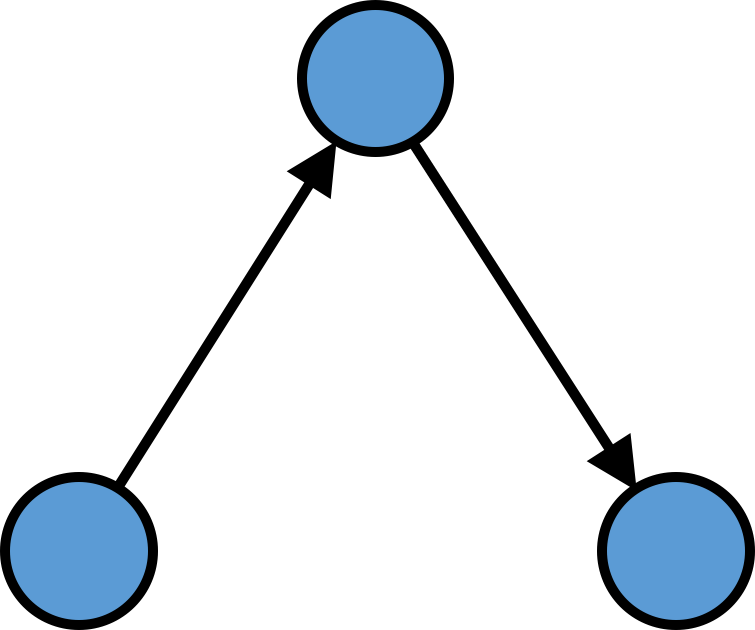
\includegraphics[width=0.4\linewidth]{Images/TwoPath} \end{minipage}        		& \begin{tabular}[c]{l}Tendency for ties to form as part of simple path formations. \end{tabular} \\ \\
		AinS (popularity spread)      	& \begin{minipage}{.2\textwidth} \centering 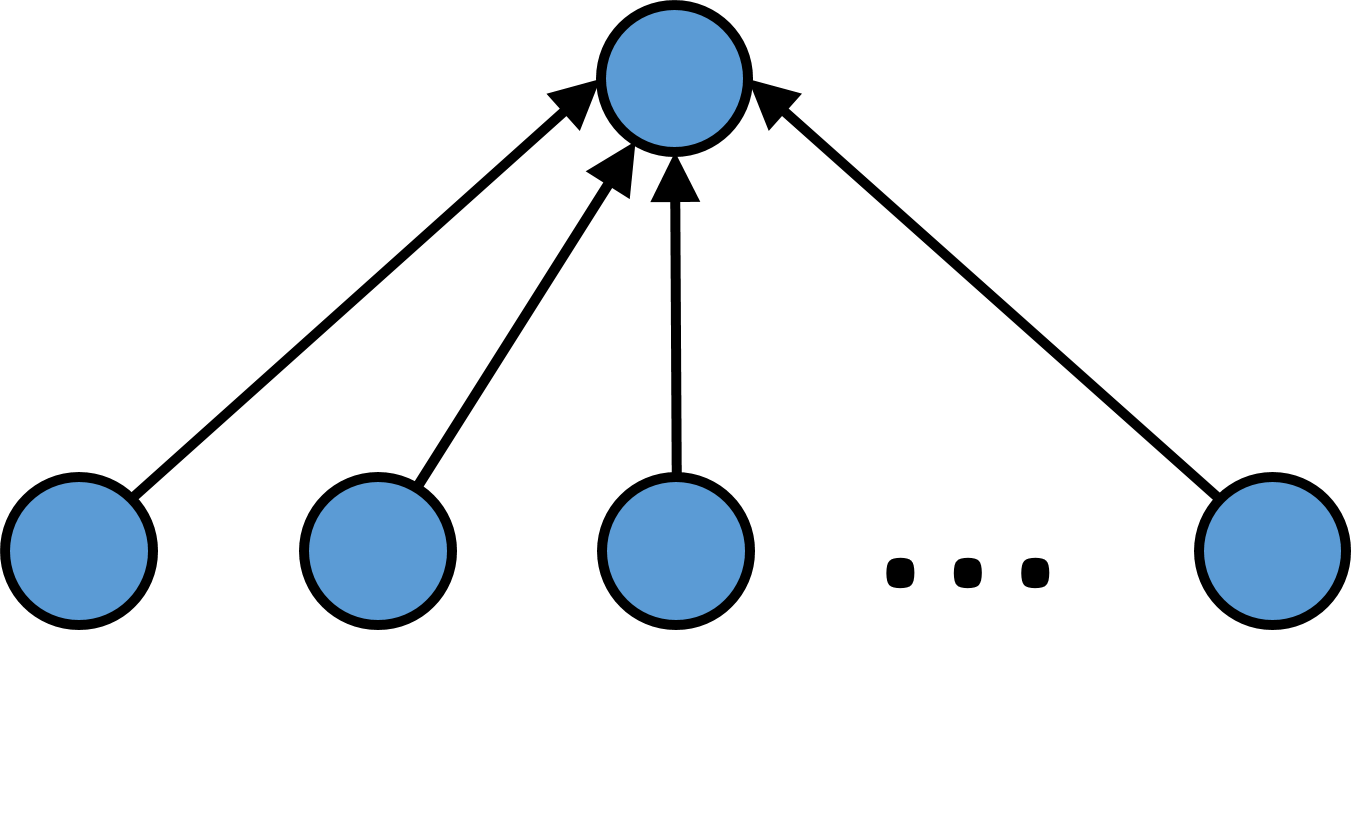
\includegraphics[width=0.6\linewidth]{Images/AinS} \end{minipage}        			& \begin{tabular}[c]{l}Propensity for dispersion in the in-degree distribution,\\ indicating there are a few highly popular actors. \end{tabular} \\ \\
		AoutS (activity spread)       	& \begin{minipage}{.2\textwidth} \centering 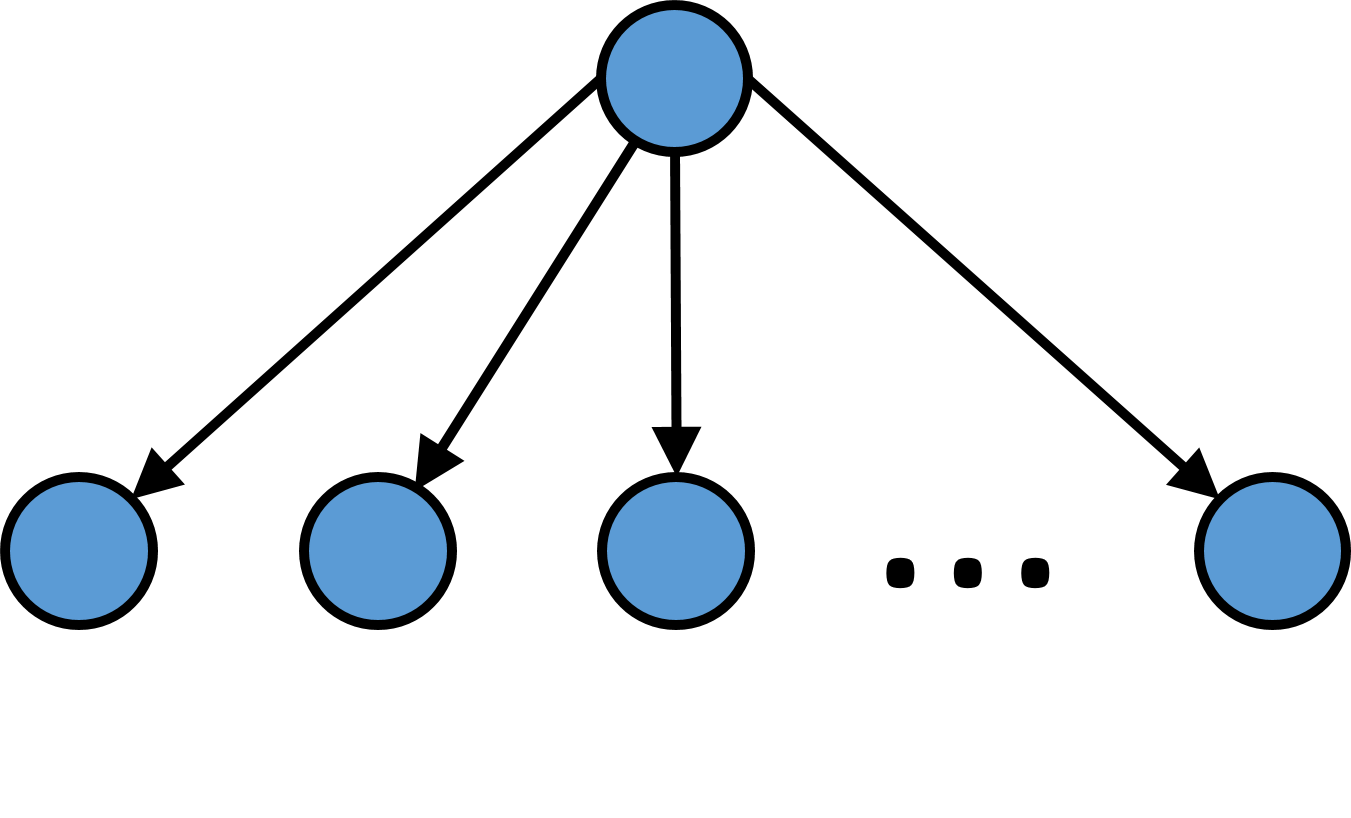
\includegraphics[width=0.6\linewidth]{Images/AoutS} \end{minipage}  				& \begin{tabular}[c]{l}Propensity for dispersion in the out-degree distribution,\\ indicating there are a few highly active actors. \end{tabular}  \\ \\
		AT-T (path closure)           	& \begin{minipage}{.2\textwidth} \centering 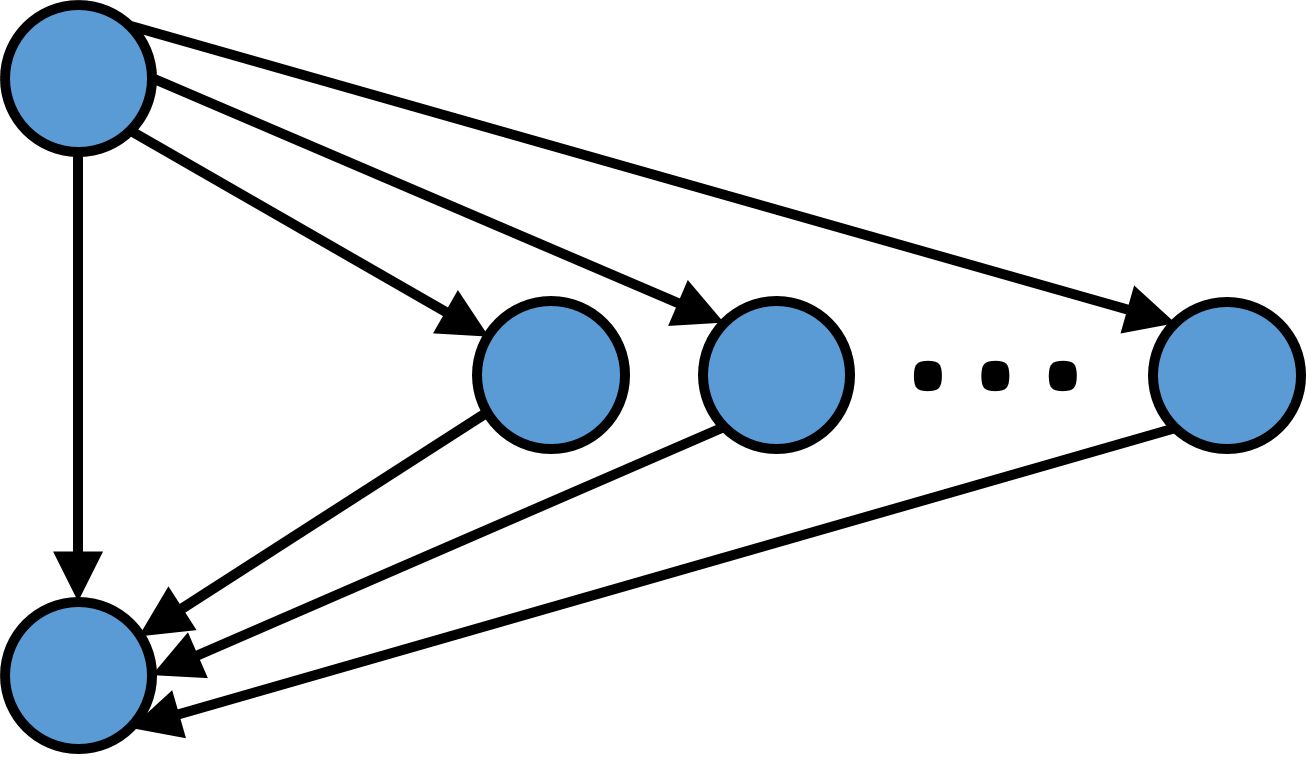
\includegraphics[width=0.6\linewidth]{Images/AT-T} \end{minipage}        			& \begin{tabular}[c]{l}Propensity for ties to form as part of transitive triad or a\\ multiple transitive configuration. \end{tabular} \\ \\
		AT-C (cyclic closure)         	& \begin{minipage}{.2\textwidth} \centering 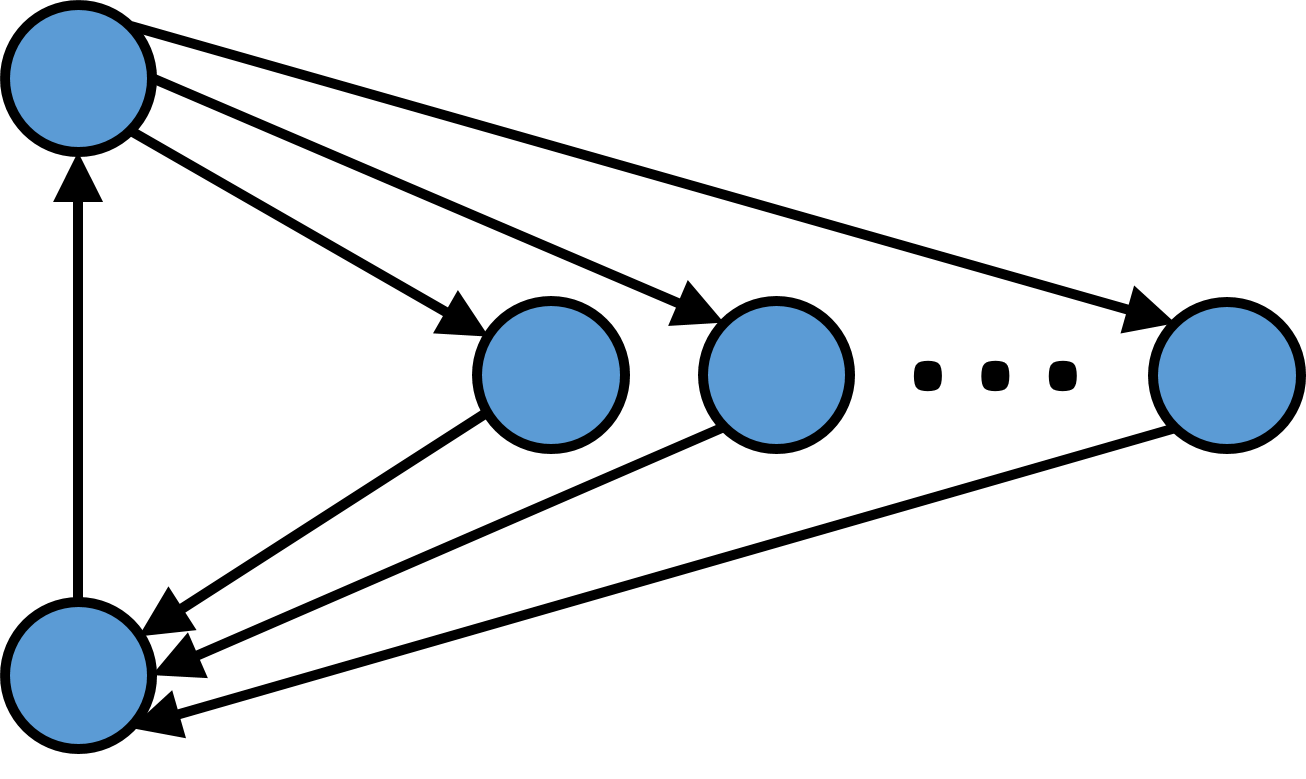
\includegraphics[width=0.6\linewidth]{Images/AT-C} \end{minipage}        			& \begin{tabular}[c]{l}Propensity for ties to form as part of a cyclic triad or a\\ multiple cyclic configuration. \end{tabular} \\ \\
		A2P (multiple connectivity)   	& \begin{minipage}{.2\textwidth} \centering 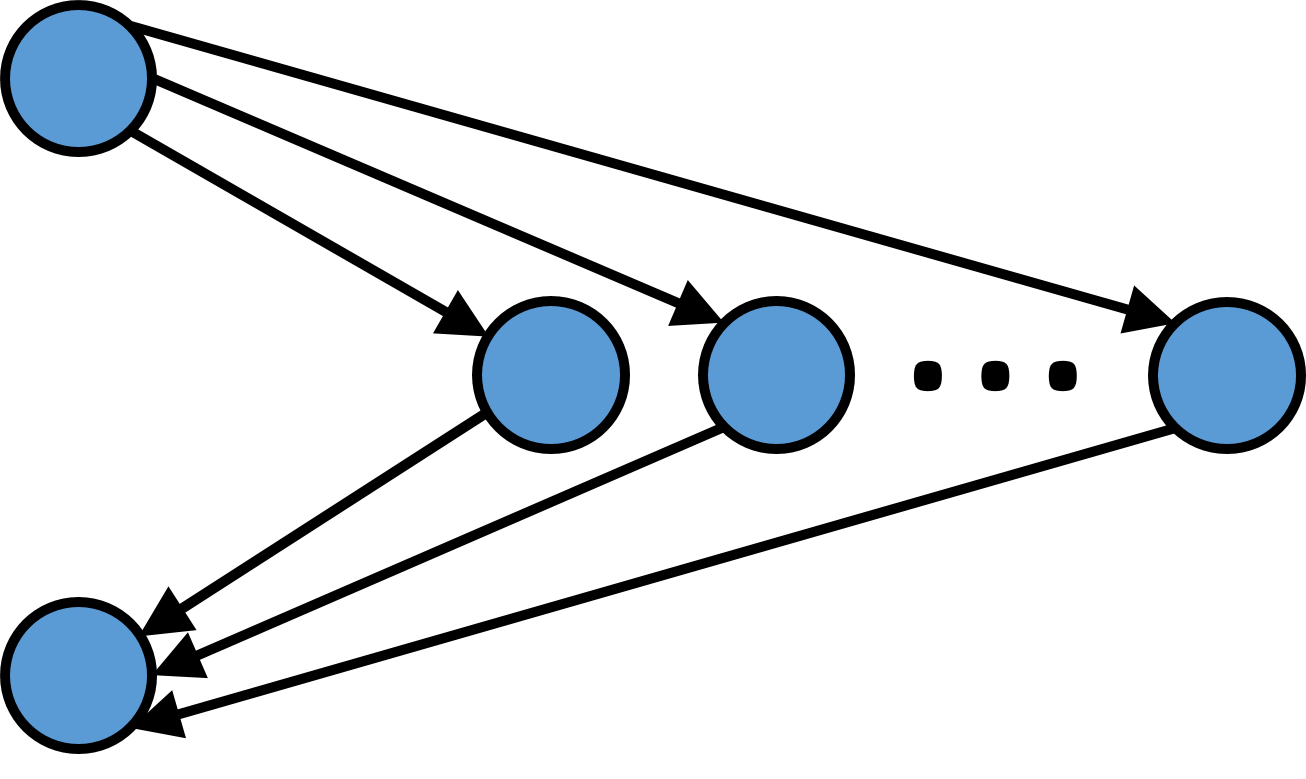
\includegraphics[width=0.6\linewidth]{Images/A2P} \end{minipage}       				& \begin{tabular}[c]{l}Propensity for ties to form as part of formations involving\\ multiple short paths between actors. \end{tabular} \\ \\
		\textbf{Actor-relation effects} & & \\
		Attribute sender              	& \begin{minipage}{.2\textwidth} \centering 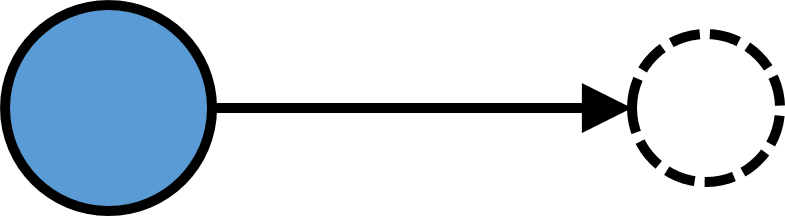
\includegraphics[width=0.4\linewidth]{Images/Sender} \end{minipage}        			& \begin{tabular}[c]{l}Propensity for a tie to be directed from an actor with a\\ particular attribute. \end{tabular} \\ \\
		Attribute receiver             	& \begin{minipage}{.2\textwidth} \centering 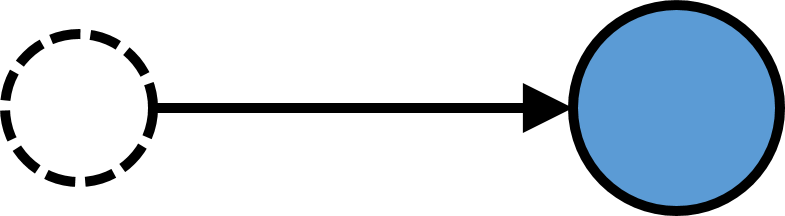
\includegraphics[width=0.4\linewidth]{Images/Receiver} \end{minipage}        		& \begin{tabular}[c]{l}Propensity for a tie to be directed toward an actor with a\\ particular attribute. \end{tabular} \\ \\
		Attribute match               	& \begin{minipage}{.2\textwidth} \centering 
\includegraphics[width=0.4\linewidth]{Images/Match} \end{minipage}       			& \begin{tabular}[c]{l}Propensity for a tie to form between actors with the same\\ categorical attribute.\end{tabular} \\ \\
		Attribute mismatch reciprocity 	& \begin{minipage}{.2\textwidth} \centering 
\includegraphics[width=0.4\linewidth]{Images/MisMatchReciprocity} \end{minipage}  	& \begin{tabular}[c]{l}Propensity for a tie to form between actors with a\\ non-matching categorical attribute.\end{tabular} \\ \\
		Attribute difference          	& \begin{minipage}{.2\textwidth} \centering 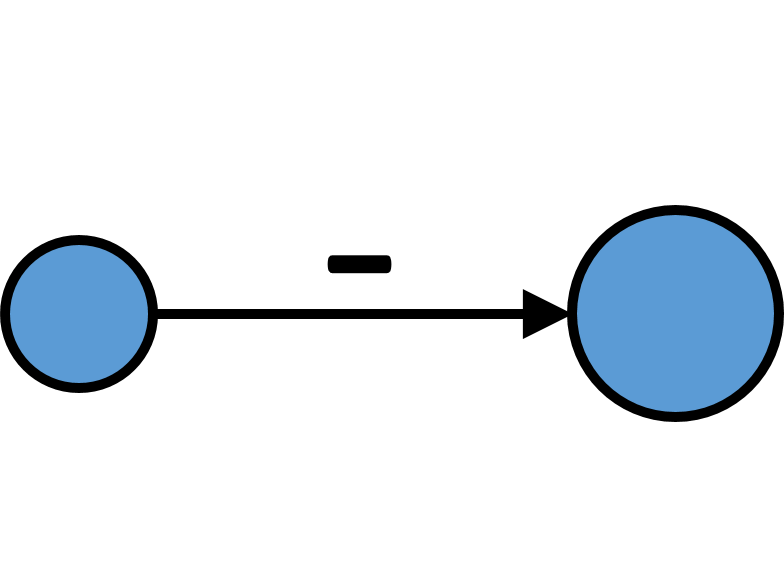
\includegraphics[width=0.4\linewidth]{Images/Difference} \end{minipage}       		& \begin{tabular}[c]{l}Propensity for a tie to form between actors with a similar\\ continuous attribute. \end{tabular} \\ \\
		Attribute product             	& \begin{minipage}{.2\textwidth} \centering 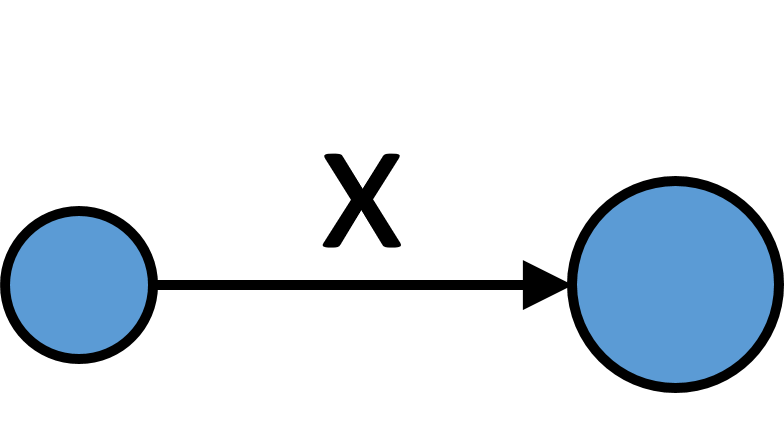
\includegraphics[width=0.4\linewidth]{Images/Product} \end{minipage}        		& \begin{tabular}[c]{l}Propensity for a tie to form between actors who both score\\ highly on the same continuous attribute. \end{tabular} \\ \\
		\textbf{Actor-brokerage effects} & & \\
		b\textsubscript{O} (liaison role)			      	&  \begin{minipage}{.2\textwidth} \centering 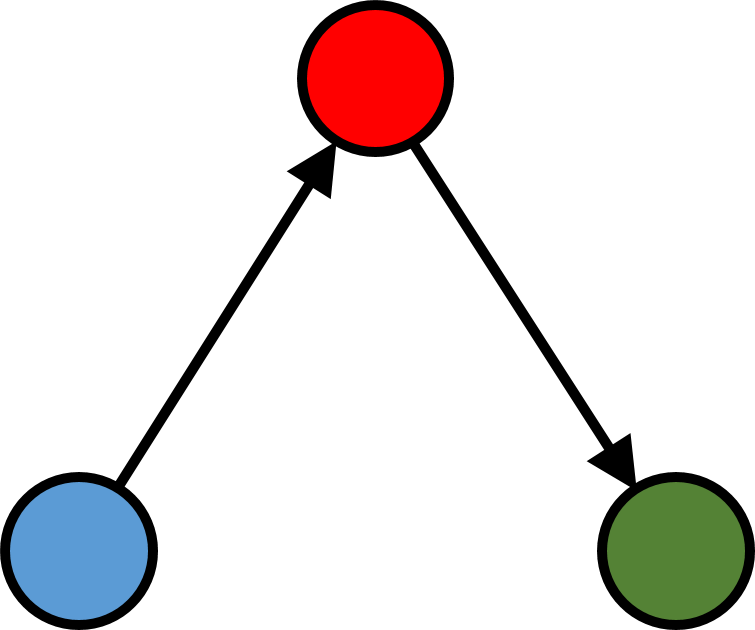
\includegraphics[width=0.4\linewidth]{Images/b_O} \end{minipage}   & \begin{tabular}[c]{l}Propensity to have brokers who mediate communication\\ between two individuals from different groups, neither of\\ which they belong to.\end{tabular}\\ \\
		b\textsubscript{IO} (representative role)		   	& \begin{minipage}{.2\textwidth} \centering 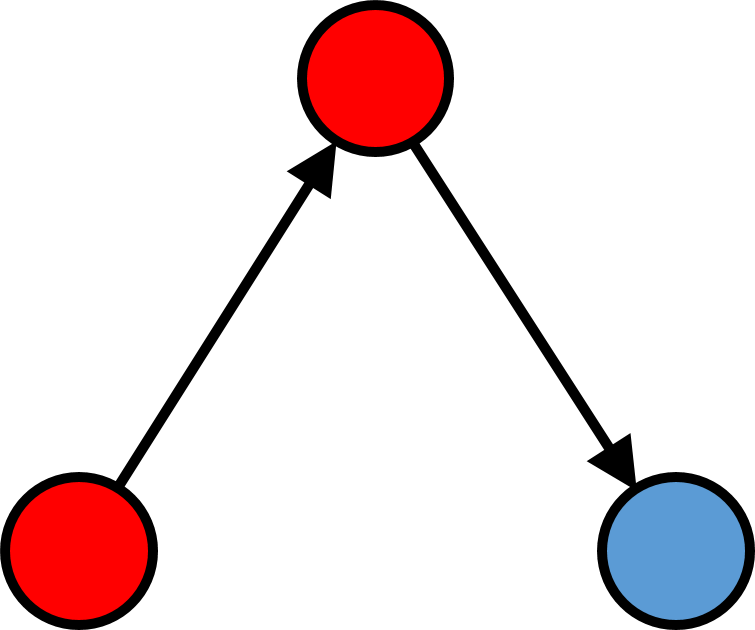
\includegraphics[width=0.4\linewidth]{Images/b_IO} \end{minipage}   & \begin{tabular}[c]{l}Propensity to have brokers who mediate communication\\ from in-group members to out-group members.\end{tabular}\\ \\
		b\textsubscript{OI} (gatekeeper role) 				& \begin{minipage}{.2\textwidth} \centering 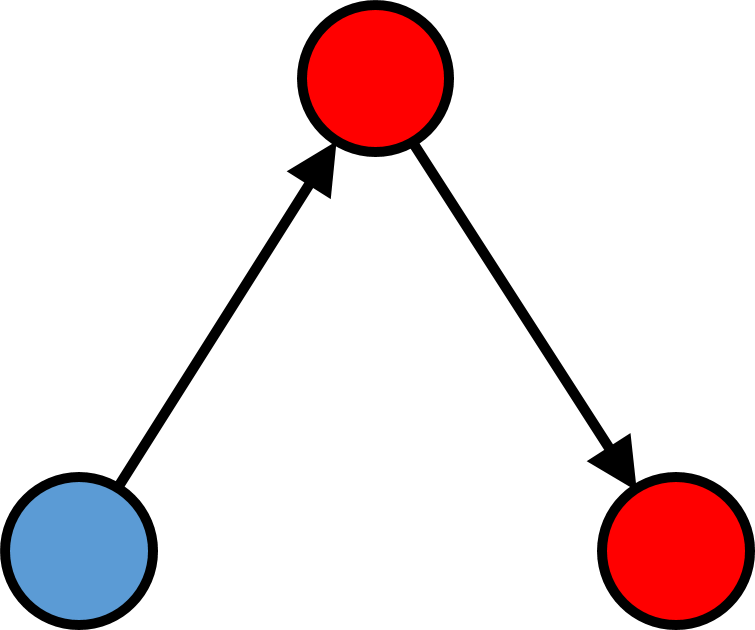
\includegraphics[width=0.4\linewidth]{Images/b_OI} \end{minipage}   & \begin{tabular}[c]{l}Propensity to have brokers who mediate communication\\ from out-group members to in-group members. \end{tabular}\\ \\
		w\textsubscript{O} (itinerant broker)			&  \begin{minipage}{.2\textwidth} \centering 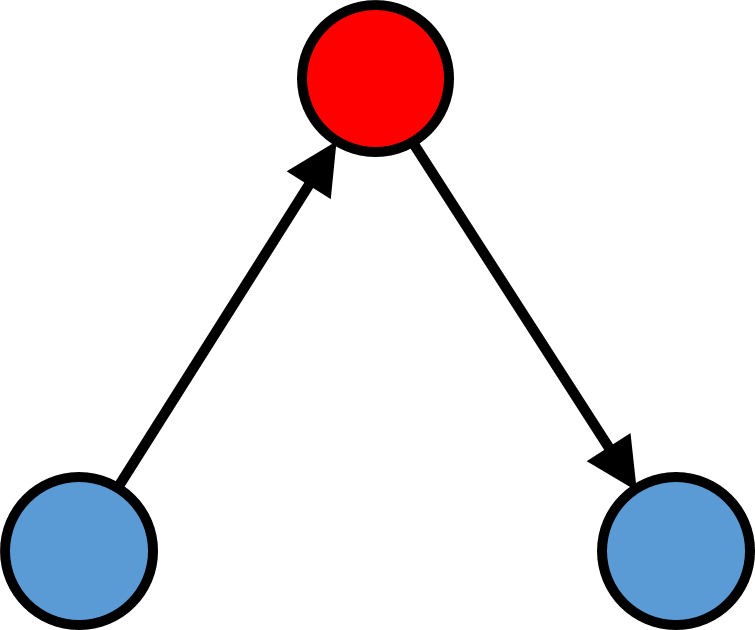
\includegraphics[width=0.4\linewidth]{Images/w_O} \end{minipage}   & \begin{tabular}[c]{l}Propensity to have brokers who mediate communication\\ between two individuals from a single group to which they\\ do not belong. \end{tabular}\\ 
		w\textsubscript{I} (coordination role)				& \begin{minipage}{.2\textwidth} \centering 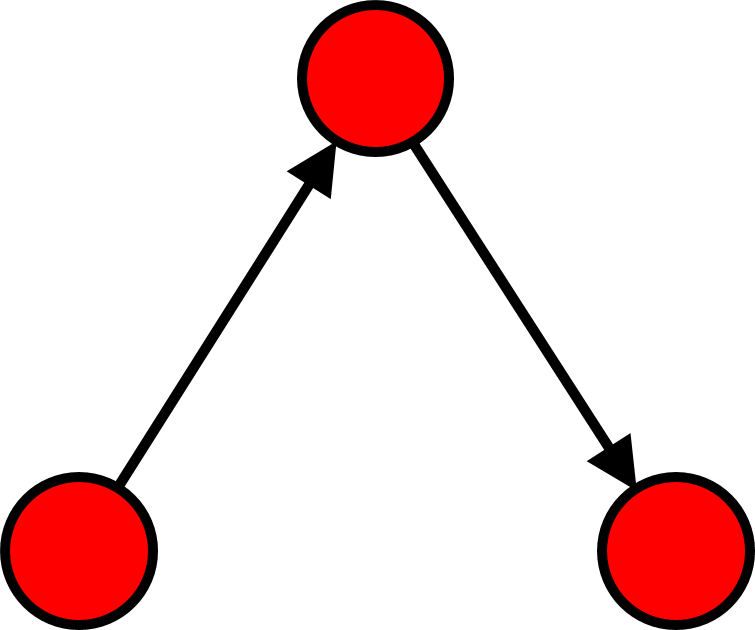
\includegraphics[width=0.4\linewidth]{Images/w_I} \end{minipage}    & \begin{tabular}[c]{l}Propensity to have brokers who mediate communication\\ between two individuals from his or her own group. \end{tabular}\\ \\	
		\textbf{Network covariate effects} & & \\
		Dyadic covariate             	& \begin{minipage}{.2\textwidth} \centering 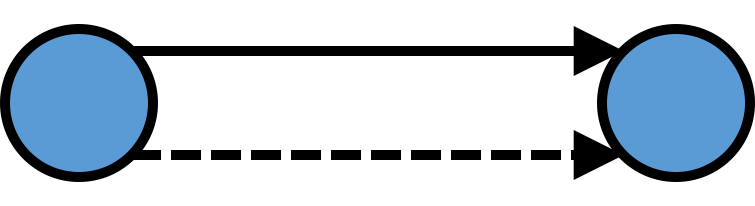
\includegraphics[width=0.4\linewidth]{Images/DyadicCovariate} \end{minipage}    	& \begin{tabular}[c]{l}Propensity for a tie of one type to form from one actor to\\ another if a tie of another type is already present, though\\ the covariate network is fixed (i.e. exogenous) in the\\ model, and so cannot vary. \end{tabular} \\\bottomrule                                                                                                       
	\end{tabular}
\end{table}

\subsubsection{Brokerage roles}

\begin{table}[]
	\small
	\centering
	\caption{Gould-Fernandez brokerage roles}
	\label{gf_params}
	\begin{tabular}{@{}lcl@{}}
		\toprule
		\multicolumn{1}{c}{Role} & \multicolumn{1}{c}{Graphic} & \multicolumn{1}{c}{Explanation} \\ \midrule
		b\textsubscript{O} (liaison role)			&  \begin{minipage}{.2\textwidth} \centering 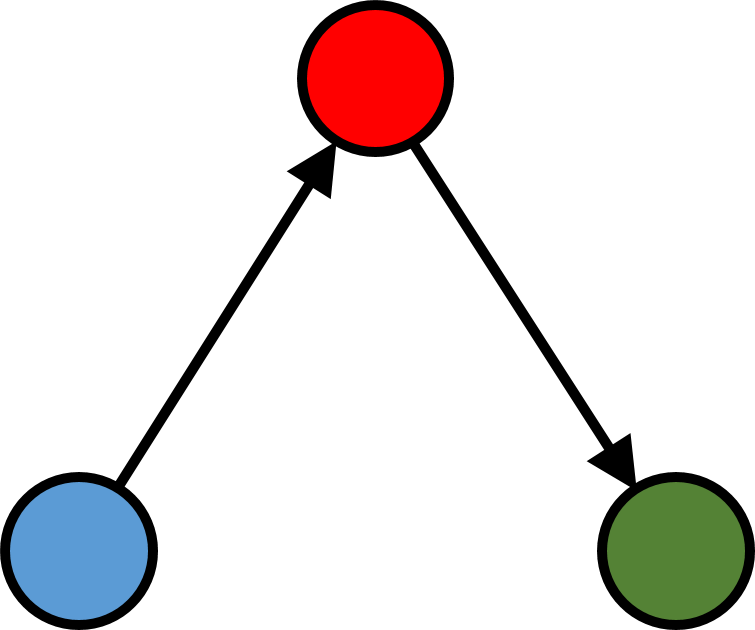
\includegraphics[width=0.4\linewidth]{Images/b_O} \end{minipage}	& \begin{tabular}[c]{l}Broker mediates contact between two\\ individuals from different groups,\\ neither of which is the group to\\ which he or she belongs.\end{tabular}\\ [10ex]
		b\textsubscript{IO} (representative role)	& \begin{minipage}{.2\textwidth} \centering 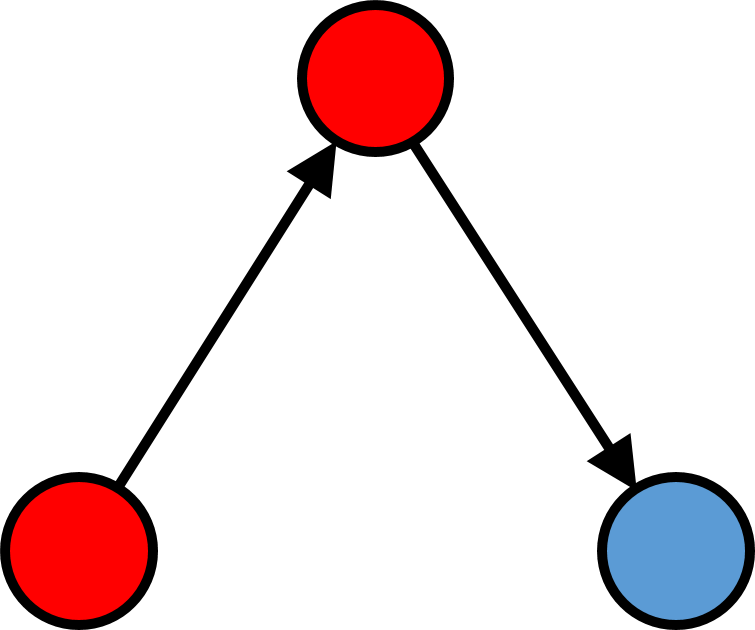
\includegraphics[width=0.4\linewidth]{Images/b_IO} \end{minipage}   & \begin{tabular}[c]{l}Broker mediates an outgoing contact\\ from an in-group member to an\\ out-group member.\end{tabular}\\ [10ex]
		b\textsubscript{OI} (gatekeeper role)		& \begin{minipage}{.2\textwidth} \centering 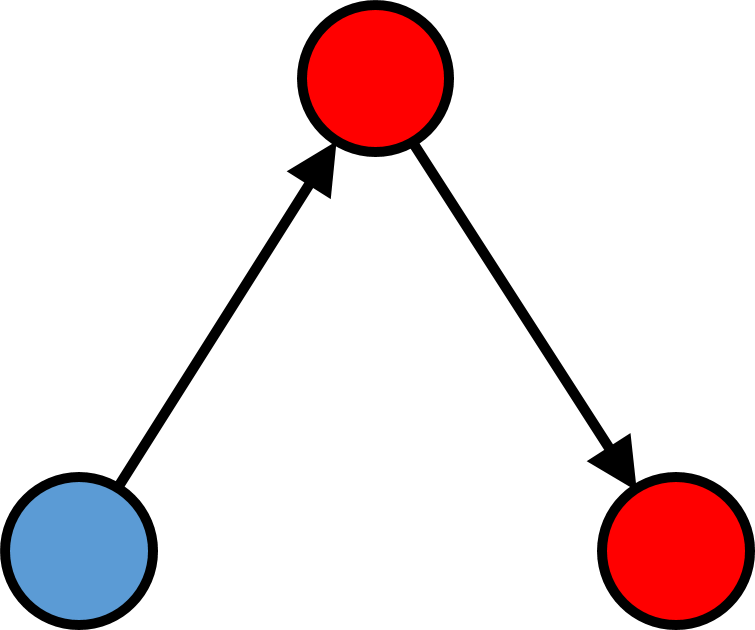
\includegraphics[width=0.4\linewidth]{Images/b_OI} \end{minipage}   & \begin{tabular}[c]{l}Broker mediates an incoming contact\\ from an out-group member to an\\ in-group member. \end{tabular}\\ [10ex]
		w\textsubscript{O} (itinerant broker)		&  \begin{minipage}{.2\textwidth} \centering 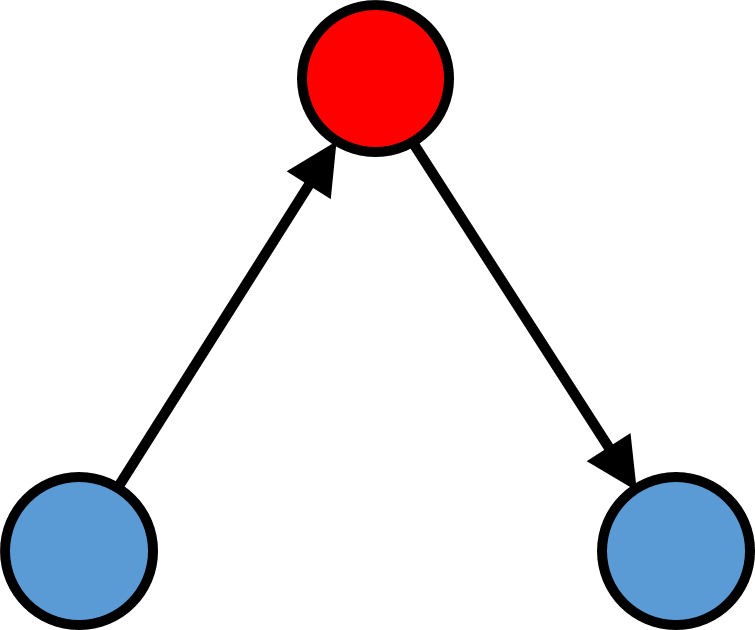
\includegraphics[width=0.4\linewidth]{Images/w_O} \end{minipage}   & \begin{tabular}[c]{l}Broker mediates contact between two\\ individuals from a single group to\\ which he or she does not belong. \end{tabular}\\ [10ex]
		w\textsubscript{I} (coordination role)		& \begin{minipage}{.2\textwidth} \centering 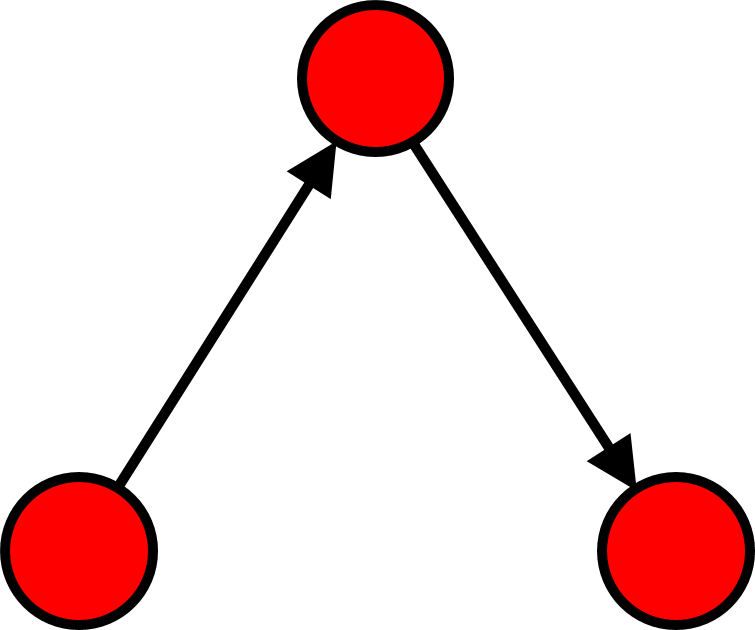
\includegraphics[width=0.4\linewidth]{Images/w_I} \end{minipage}    & \begin{tabular}[c]{l}Broker mediates contact between two\\ individuals from his or her own\\ group. \end{tabular}\\ 
		\bottomrule
	\end{tabular}
\end{table}

Experience is also identified as being a main source of tacit knowledge creation \citep{nonaka1995knowledge,sternberg1999tacit}.

\section{Qualitative procedures}



% 



% \begin{table}[]
% \centering
% \caption{My caption}
% \label{tab:approach}
% \begin{adjustbox}{width = \textwidth}
% \begin{tabular}{@{}lccc@{}}
% \toprule
%  & Postivisim & Constructivism & Pragmatism \\ \midrule
% Connection of theory and data & Deduction & Induction & Abduction \\
% Relationship to research process & Objectivity & Subjectivity & Intersubjectivity \\
% Inference from data & Generality & Context & Transferability \\ \bottomrule
% \end{tabular}
% \end{adjustbox}
% \end{table}

% \begin{table}[]
% \centering
% \caption{Positivist vs. constructivist epistemologies \citep{easterby2015management}.}
% \label{tab:epistemology}
% \begin{adjustbox}{width = \textwidth}
% \begin{tabular}{@{}lll@{}}
% \toprule
% \multicolumn{1}{c}{Aspect} & \multicolumn{1}{c}{Positivism} & \multicolumn{1}{c}{Constructivism} \\ \midrule
% The observer & Must be independent & Is part of what is being observed \\
% Human interests & Should be irrelevant & Are the main drivers of science \\
% Explanations & Must demonstrate causality & Aim to increase the general understanding of the situation \\
% Research progresses through & Hypotheses and deductions & Gathering rich data from which ideas are induced \\
% Concepts & Need to be defined so they can be measured & Should incorporate stakeholder concepts \\
% Units of analysis & Should be reduced to the simplest terms & May account for complexity of whole situations \\
% Generalisation through & Statistical probability & Theoretical abstraction \\
% Sampling requires & Large numbers selected randomly & Small number of cases,chosen for specific reasons \\ \bottomrule
% \end{tabular}
% \end{adjustbox}
% \end{table}